\documentclass[11pt]{article}

\usepackage[margin=1in]{geometry}
\usepackage{graphicx}
\usepackage{booktabs}
\usepackage{longtable}
\usepackage{xcolor}
\usepackage{listings}
\usepackage{hyperref}
\usepackage{amsmath}
\usepackage{amssymb}
\usepackage{enumitem}
\usepackage{fancyhdr}
\usepackage{caption}
\setlength{\headheight}{14pt}

\graphicspath{{diagrams/}}

\hypersetup{
    colorlinks=true,
    linkcolor=blue!50!black,
    urlcolor=blue!50!black,
    citecolor=blue!50!black,
    pdftitle={Hybrid FTP -- Technical Report},
}

\lstdefinestyle{code}{
    basicstyle=\ttfamily\small,
    breaklines=true,
    frame=single,
    columns=fullflexible,
    backgroundcolor=\color{gray!8},
    commentstyle=\color{gray!60!black},
    keywordstyle=\color{blue!60!black}\bfseries,
    stringstyle=\color{green!40!black},
}
\lstset{style=code}

\pagestyle{fancy}
\fancyhf{}
\fancyhead[L]{Hybrid FTP -- Technical Report}
\fancyhead[R]{\thepage}
\renewcommand{\headrulewidth}{0.4pt}

\title{\textbf{Hybrid FTP Application}\\[4pt]\large Design and Implementation Technical Report}
\author{%
  % TODO(team): add student IDs
  Doan Cong Pho (ID: \_\_\_\_\_\_\_\_) \and Le Kim Chau (ID: \_\_\_\_\_\_\_\_)
}
\date{Internetworking Protocol -- Project 1}

\begin{document}
\maketitle
\tableofcontents
\newpage

% ============================================================
\section{Application Scenario \& Protocol Interaction}
% ============================================================

\subsection{Overview}

The Hybrid FTP application decouples the control plane from the data plane, mirroring
RFC~959's architectural philosophy while adapting it to a connectionless UDP data
channel:

\begin{itemize}
    \item \textbf{Control channel} -- TCP, port 2121. One command/reply per line,
          CRLF-terminated, three-digit FTP-style reply codes (Section 2.3 of the
          project spec).
    \item \textbf{Data channel} -- UDP. File payload and (Advanced Level) directory
          listing text, framed with a 9-byte custom header (Section~2 of this report).
          Because UDP provides no delivery guarantee, a from-scratch reliability
          sub-protocol (Go-Back-N, Excellent Level) is layered on top, opt-in via
          \texttt{config.ini}.
\end{itemize}

Three data-channel operating modes are supported (Advanced Level): \textbf{FIXED}
(Basic Level default -- a single, server-wide UDP socket, address learned via one
\texttt{HELLO} datagram), \textbf{PASSIVE} (\texttt{PASV} -- server opens a
per-session ephemeral socket and announces it), and \textbf{ACTIVE} (\texttt{PORT} --
client announces its own address; the server still opens a per-session socket and
reports its own port back, a deliberate deviation from RFC~959 discussed in
Section~3.4).

\subsection{Sequence Diagrams}

Figure~\ref{fig:seq-full} traces the complete lifecycle of one session: TCP
handshake, authentication, the FIXED-mode UDP address-learning handshake, an upload
(\texttt{STOR}) using the Go-Back-N reliable-UDP layer -- including one simulated
packet loss and its recovery -- and end-to-end hash verification.

\begin{figure}[htbp]
    \centering
    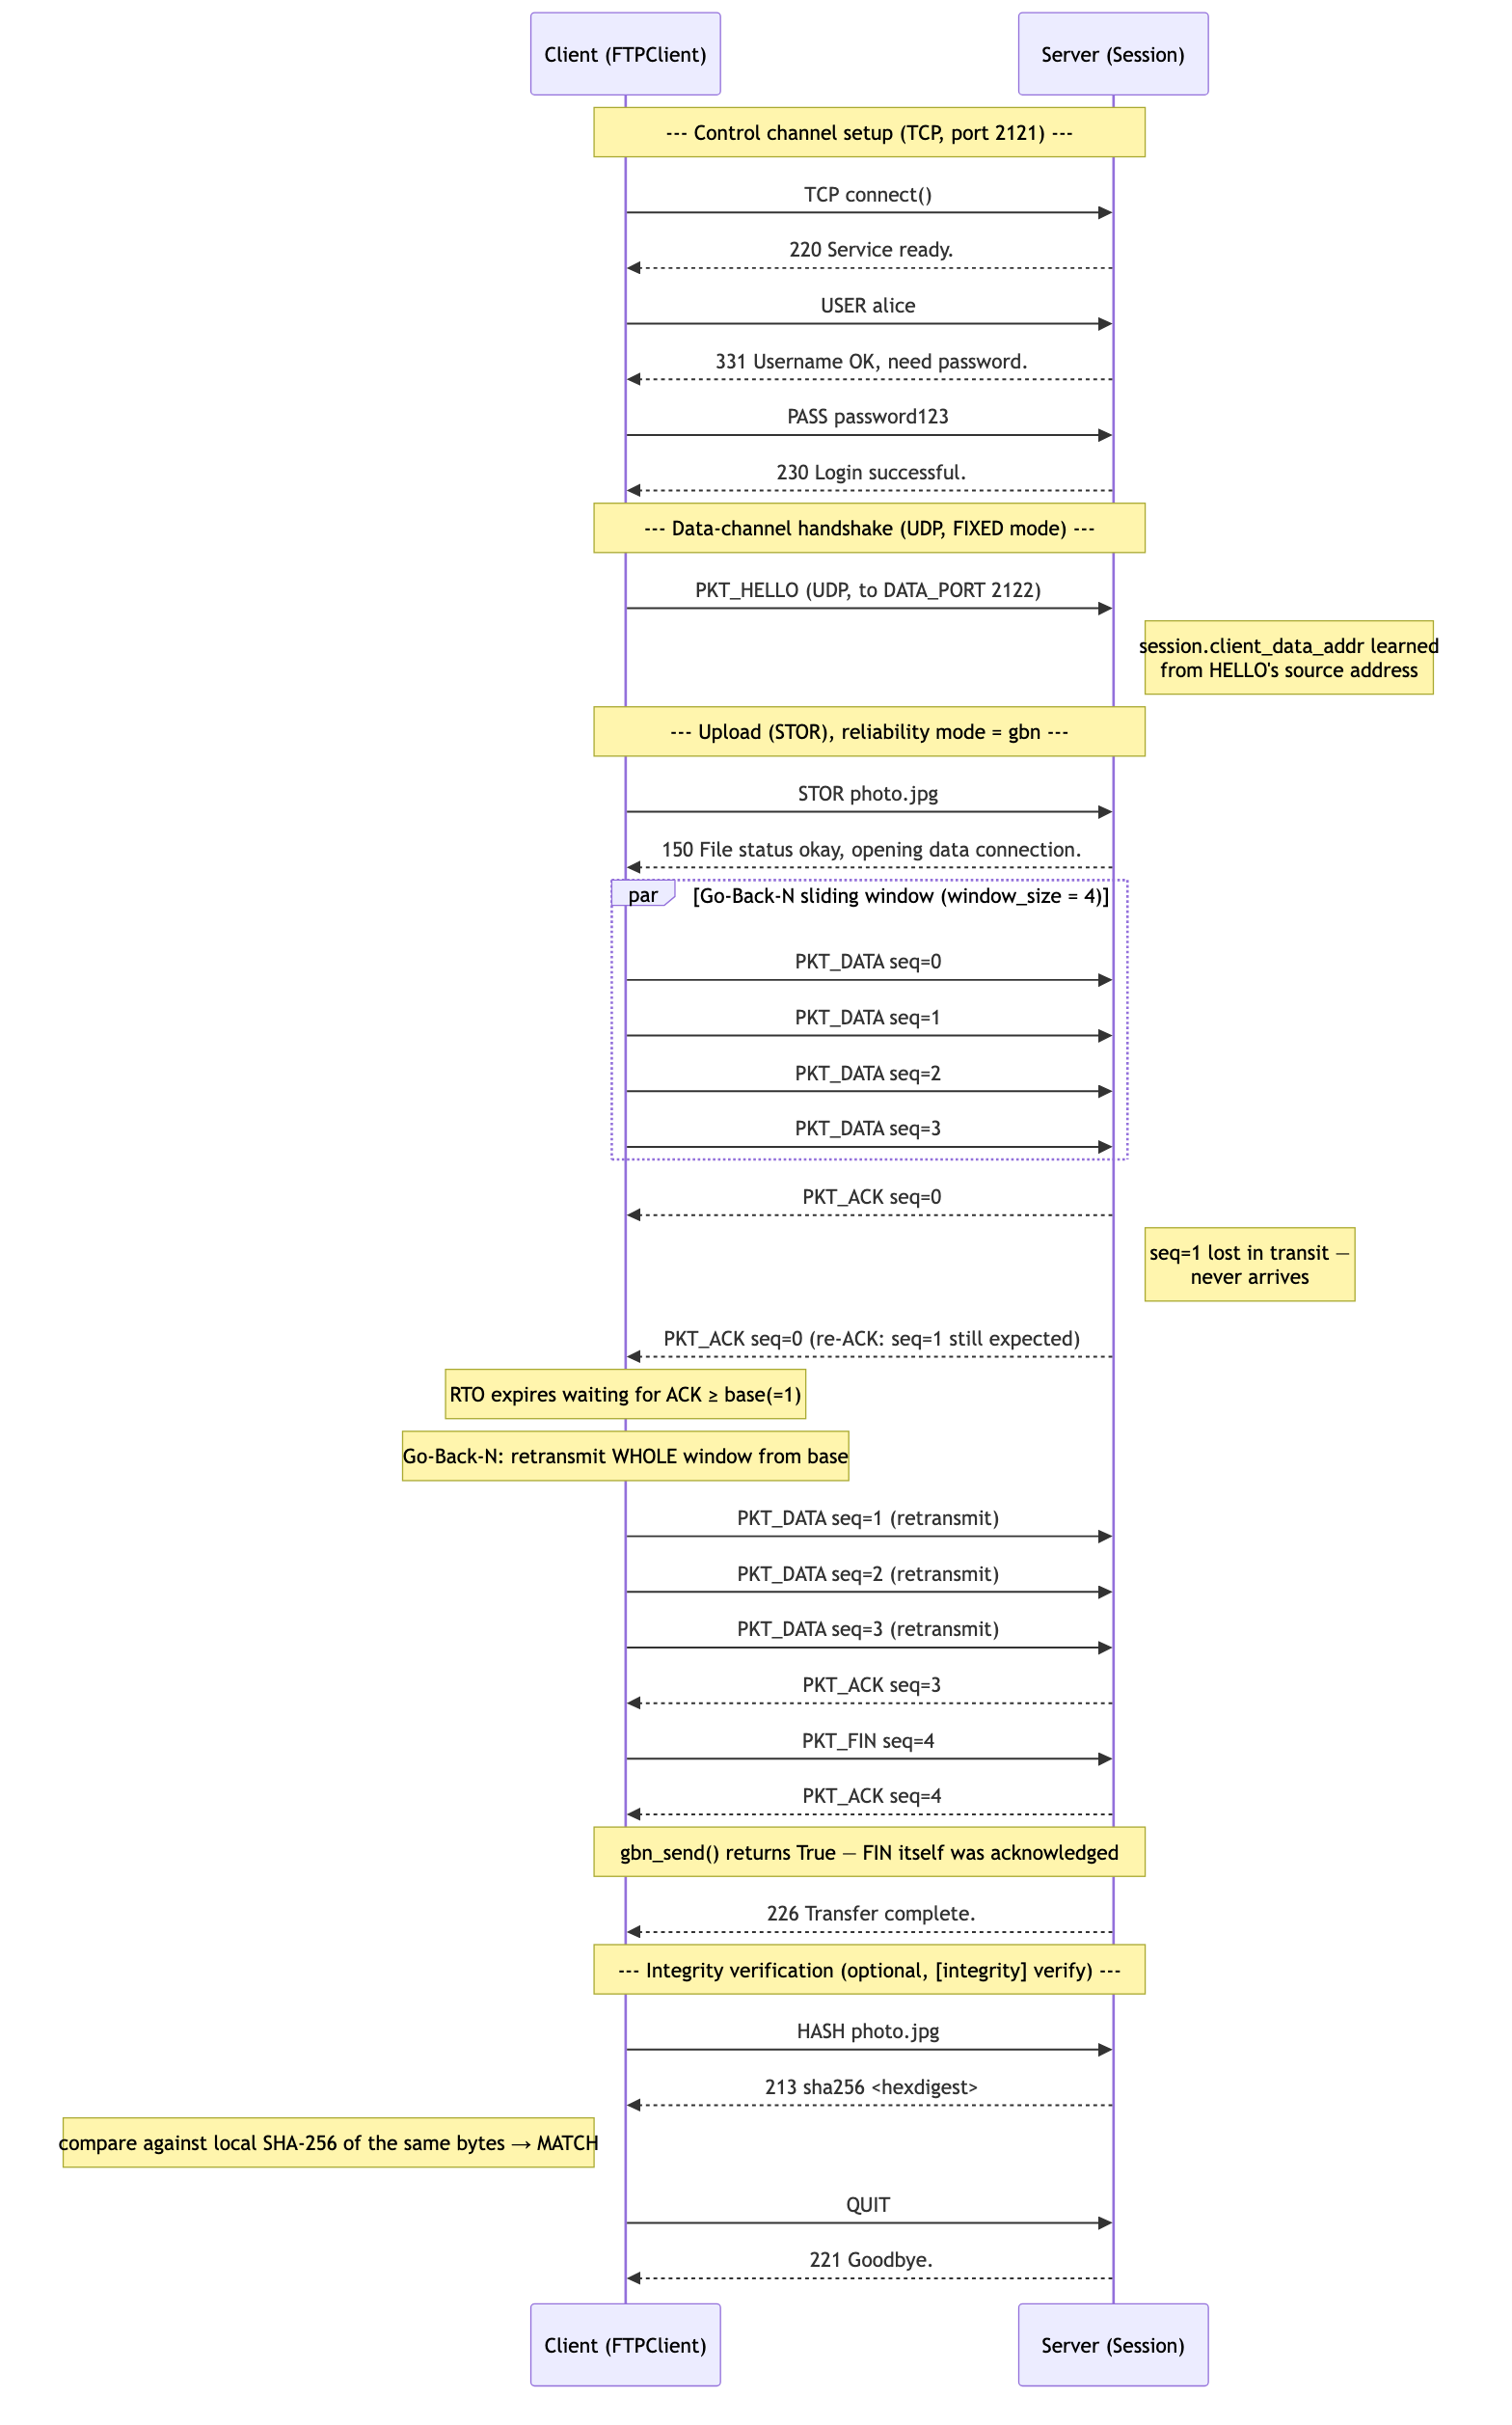
\includegraphics[width=0.85\textwidth,height=0.85\textheight,keepaspectratio]{01_sequence_full_lifecycle.png}
    \caption{Full TCP + UDP session lifecycle, including a Go-Back-N retransmission
             after a simulated packet loss on \texttt{seq=1}.}
    \label{fig:seq-full}
\end{figure}

\clearpage
Figure~\ref{fig:seq-active-passive} details the two Advanced Level mode-negotiation
paths side by side.

\begin{figure}[htbp]
    \centering
    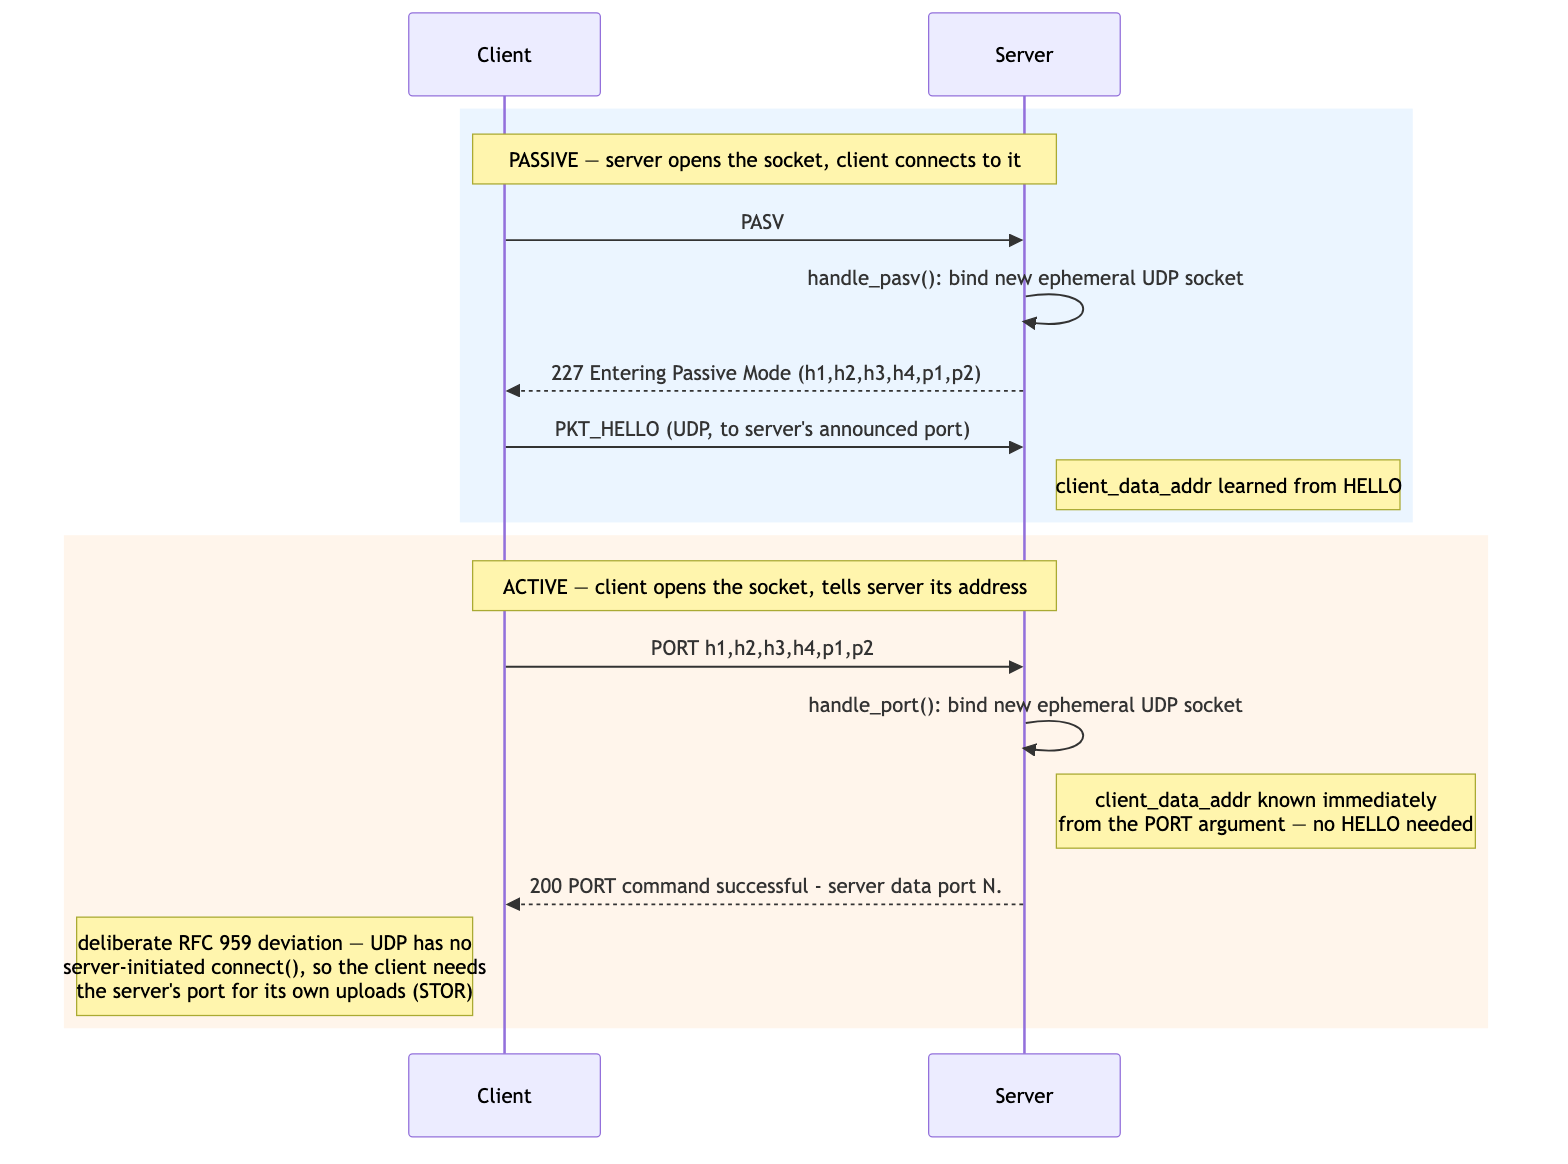
\includegraphics[width=0.8\textwidth,height=0.8\textheight,keepaspectratio]{02_sequence_active_passive.png}
    \caption{Passive (\texttt{PASV}) vs. Active (\texttt{PORT}) mode negotiation.}
    \label{fig:seq-active-passive}
\end{figure}

\clearpage
% ============================================================
\section{Project-Wide Data Structures}
% ============================================================

\subsection{TCP Control-Channel Line Protocol}

The control channel carries no binary framing -- every message is a single
UTF-8/ASCII line terminated by \texttt{"\textbackslash r\textbackslash n"}
(CRLF), matching RFC~959. Both directions use it: client $\to$ server commands
(e.g. \texttt{STOR photo.jpg}) and server $\to$ client replies (e.g.
\texttt{226 Transfer complete.}). Table~\ref{tab:reply-codes} summarizes the reply
code categories in use (Section 2.3 of the project spec).

\begin{table}[htbp]
\centering
\caption{Server reply code categories in use}
\label{tab:reply-codes}
\begin{tabular}{@{}lp{10.5cm}@{}}
\toprule
\textbf{Code range} & \textbf{Examples used in this project} \\
\midrule
1xx & \texttt{150} File status okay, opening data connection. \\
2xx & \texttt{200} Command OK; \texttt{220} Service ready; \texttt{226} Transfer complete;
      \texttt{230} Login successful; \texttt{250} Directory changed. \\
3xx & \texttt{331} Username OK, need password. \\
4xx & \texttt{425} Can't open data connection; \texttt{426} Connection closed, transfer aborted. \\
5xx & \texttt{500}/\texttt{501} Syntax error; \texttt{502} Not implemented;
      \texttt{530} Not logged in; \texttt{550} File unavailable. \\
\bottomrule
\end{tabular}
\end{table}

\subsection{UDP Custom Packet Header}

Every UDP datagram on the data channel is framed identically, regardless of packet
type or reliability mode (\texttt{common.py}, \texttt{HEADER\_FMT = "!BII"}, network
byte order):

\begin{table}[htbp]
\centering
\caption{UDP packet header layout -- 9 bytes, followed by up to \texttt{CHUNK\_SIZE}
         (1024) bytes of payload}
\label{tab:udp-header}
\begin{tabular}{@{}lll@{}}
\toprule
\textbf{Offset} & \textbf{Field} & \textbf{Size / Type} \\
\midrule
0       & \texttt{type}     & 1 byte, unsigned (\texttt{B}) \\
1       & \texttt{seq}      & 4 bytes, unsigned (\texttt{I}) \\
5       & \texttt{checksum} & 4 bytes, unsigned (\texttt{I}) -- CRC32 of \texttt{payload} \\
9$\ldots$ & \texttt{payload} & 0--1024 bytes \\
\bottomrule
\end{tabular}
\end{table}

\begin{table}[htbp]
\centering
\caption{Packet \texttt{type} values}
\label{tab:pkt-types}
\begin{tabular}{@{}llp{8.5cm}@{}}
\toprule
\textbf{Value} & \textbf{Name} & \textbf{Meaning} \\
\midrule
0 & \texttt{PKT\_HELLO} & Client $\to$ server: ``here is my UDP address, remember it.'' \\
1 & \texttt{PKT\_DATA}  & One chunk of file/listing payload. \\
2 & \texttt{PKT\_FIN}   & Marks the end of a transfer (its own \texttt{seq} = chunk count). \\
3 & \texttt{PKT\_ACK}   & \textit{(Excellent Level)} Go-Back-N cumulative ACK; \texttt{seq}
                            is the highest correctly-received-in-order sequence number so
                            far; empty payload. \\
\bottomrule
\end{tabular}
\end{table}

Note that \texttt{PKT\_ACK} reuses the exact same 9-byte header -- no wire-format
change was needed to add reliability; only a new \texttt{type} value and an
interpretation convention for \texttt{seq}.

\subsection{Session Management Structures (Server)}

\texttt{server.py}'s \texttt{Session} class holds all per-connection state; one
instance exists per accepted TCP connection (Table~\ref{tab:session-struct}).

\begin{table}[htbp]
\centering
\caption{\texttt{Session} fields}
\label{tab:session-struct}
\begin{tabular}{@{}llp{8.7cm}@{}}
\toprule
\textbf{Field} & \textbf{Type} & \textbf{Purpose} \\
\midrule
\texttt{id}                & int             & Monotonic session ID, shown in the active-session log table. \\
\texttt{conn}               & \texttt{socket} & TCP control-channel socket. \\
\texttt{addr}                & (str, int)      & Client's TCP address. \\
\texttt{username}            & str or None     & Set by \texttt{USER}, validated by \texttt{PASS}. \\
\texttt{authenticated}       & bool            & Gates \texttt{STOR}/\texttt{RETR}/directory/mode commands. \\
\texttt{type\_mode}          & 'A' or 'I'      & ASCII vs. binary (\texttt{TYPE}). \\
\texttt{cwd}                 & str             & FTP-space current directory, starts at \texttt{"/"}. \\
\texttt{data\_mode}          & \texttt{DataMode} & \texttt{FIXED} / \texttt{ACTIVE} / \texttt{PASSIVE}. \\
\texttt{data\_sock}          & \texttt{socket} & UDP socket used for this session's data transfers. \\
\texttt{owns\_data\_sock}    & bool            & Whether \texttt{data\_sock} is a dedicated per-session
                                                   socket (ACTIVE/PASSIVE) that must be closed on cleanup,
                                                   vs. the shared FIXED-mode socket. \\
\texttt{client\_data\_addr}  & (str, int) or None & Learned via \texttt{HELLO} (FIXED/PASSIVE) or directly
                                                       from \texttt{PORT}'s argument (ACTIVE). \\
\bottomrule
\end{tabular}
\end{table}

A global, lock-protected table (\texttt{\_active\_sessions}, keyed by \texttt{Session.id})
is updated on every connect/disconnect/mode-change event and printed to the server
log -- satisfying the checklist requirement that the server log display connected
client IPs, executed commands, and an active session table (spec Section 4.5).

\subsection{Client-Side Structures}

\texttt{client.py}'s \texttt{FTPClient} class mirrors the relevant subset of session
state needed by the client: \texttt{data\_mode}, \texttt{active\_server\_port}
(learned from the server's \texttt{PORT} reply), \texttt{passive\_target} (learned
from \texttt{PASV}'s \texttt{227} reply), plus its own \texttt{conn} (TCP) and
\texttt{udp\_sock} (UDP) sockets.

\clearpage
% ============================================================
\section{Functional Workflows}
% ============================================================

\subsection{Server Thread-Dispatch Logic}

Figure~\ref{fig:flow-dispatch} shows \texttt{server.py}'s \texttt{main()} accept
loop. When \texttt{config.ini}'s \texttt{[server] threading = thread}, each accepted
connection is handed to a new \texttt{threading.Thread}; the default
\texttt{threading = single} preserves the original Basic Level synchronous loop
(one client at a time), so this is purely an opt-in Advanced Level technique.

\begin{figure}[htbp]
    \centering
    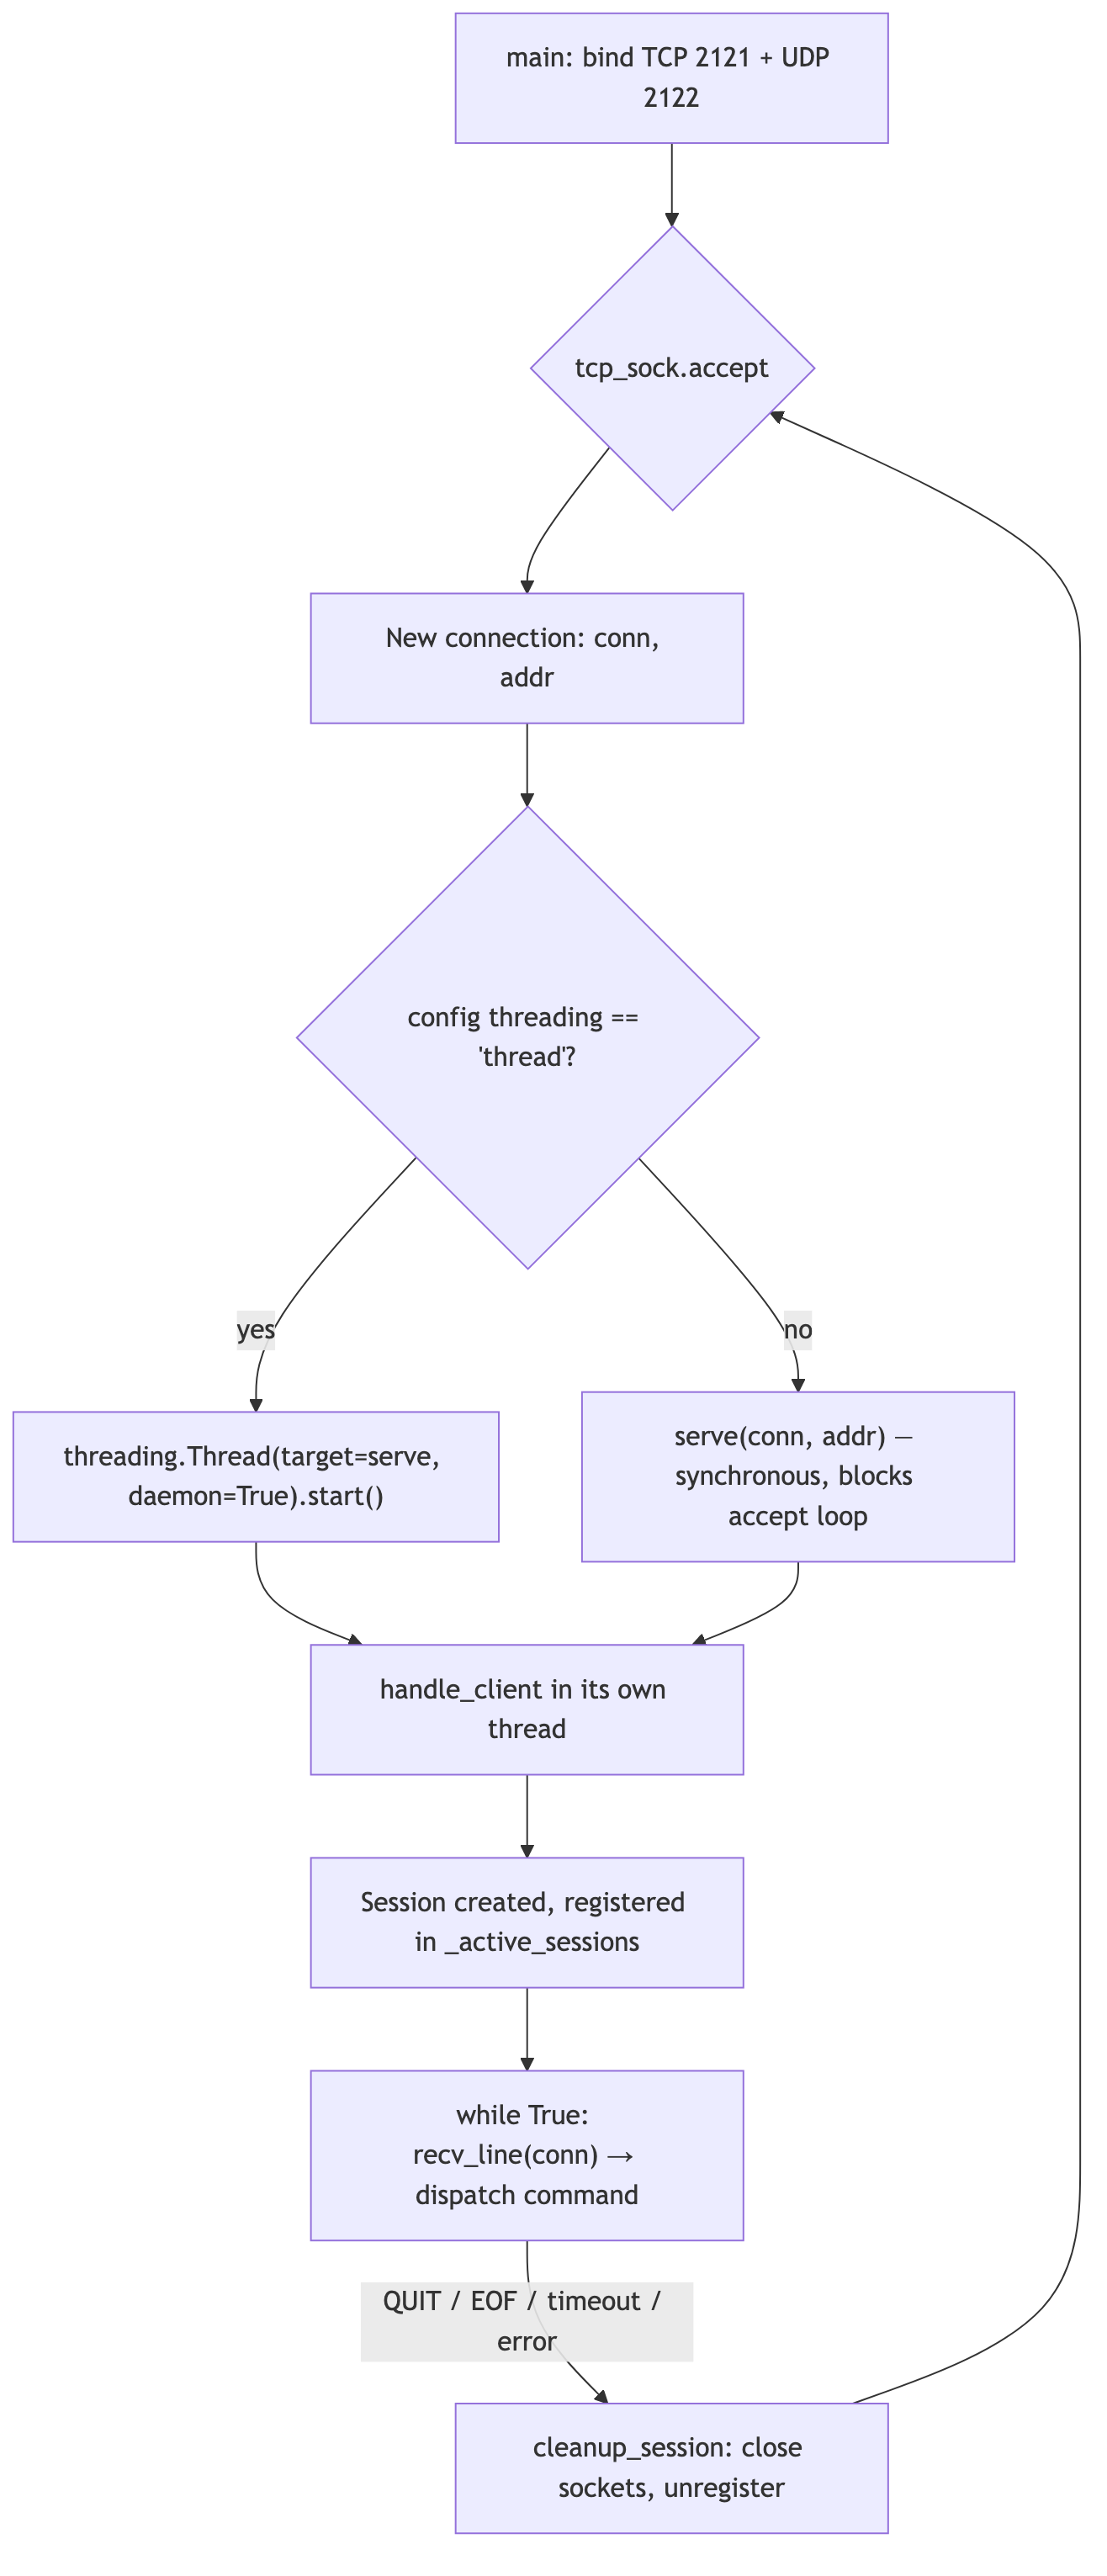
\includegraphics[width=0.75\textwidth,height=0.85\textheight,keepaspectratio]{03_flowchart_thread_dispatch.png}
    \caption{Server thread-dispatch logic.}
    \label{fig:flow-dispatch}
\end{figure}

\clearpage
\subsection{Go-Back-N Reliable-UDP State Machines}

The Excellent Level reliable-UDP layer (\texttt{common.gbn\_send()} /
\texttt{gbn\_receive()}) is implemented \emph{once} and shared identically by both
\texttt{server.py} and \texttt{client.py}, so the two ends cannot drift out of sync.
Figures~\ref{fig:flow-gbn-sender} and \ref{fig:flow-gbn-receiver} show the sender
and receiver state machines respectively.

\begin{figure}[htbp]
    \centering
    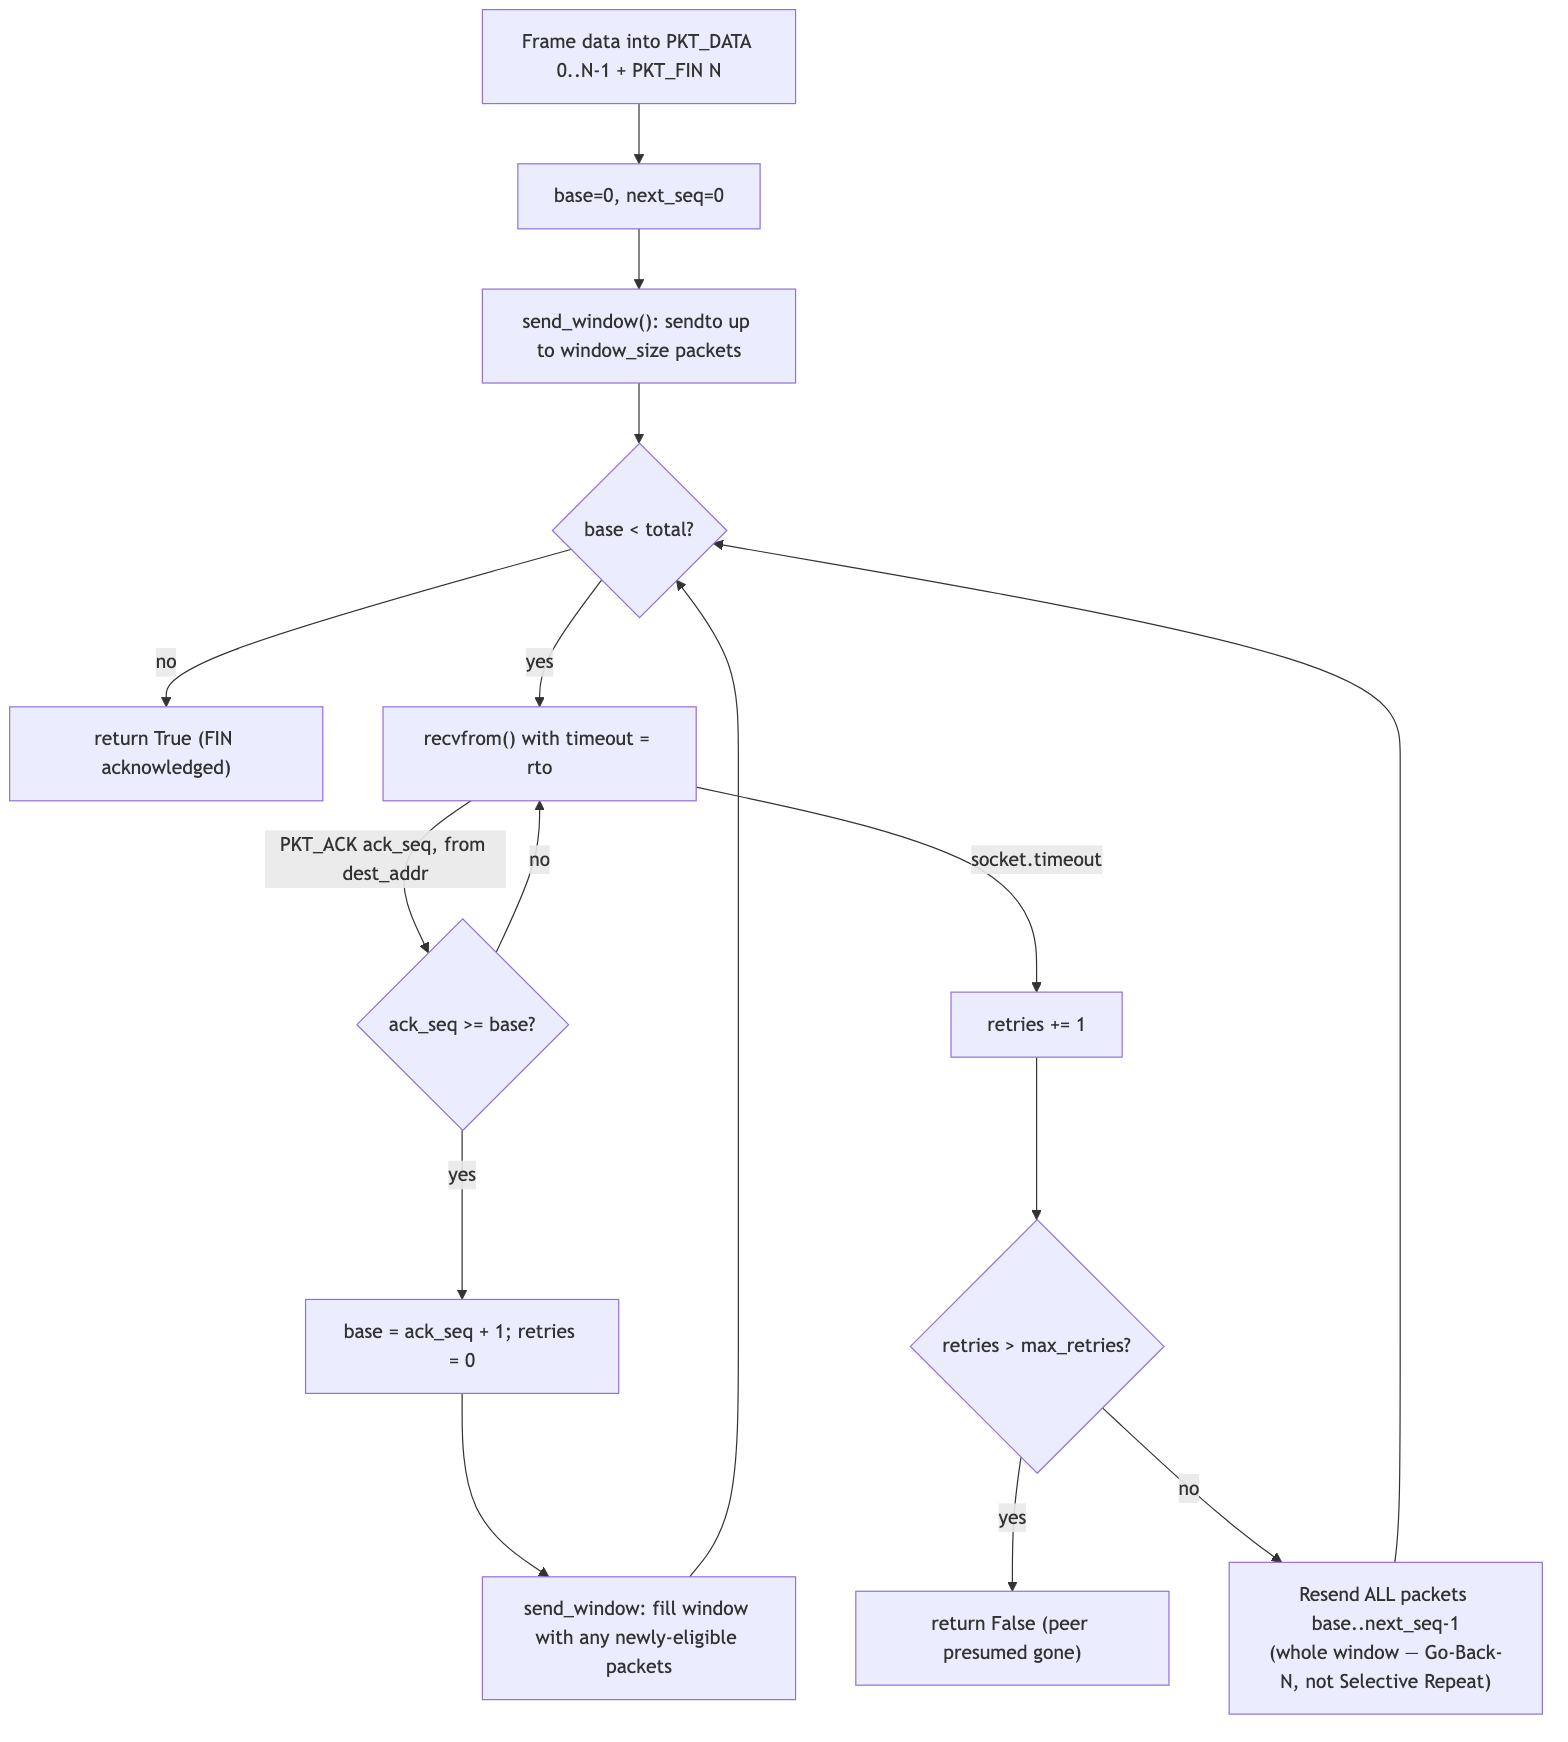
\includegraphics[width=0.78\textwidth,height=0.8\textheight,keepaspectratio]{04_flowchart_gbn_sender.png}
    \caption{Go-Back-N sender state machine. A single timer covers the oldest
             unacknowledged packet; on timeout the \emph{entire} in-flight window is
             retransmitted (the defining trait vs. Selective Repeat).}
    \label{fig:flow-gbn-sender}
\end{figure}

\clearpage
\begin{figure}[htbp]
    \centering
    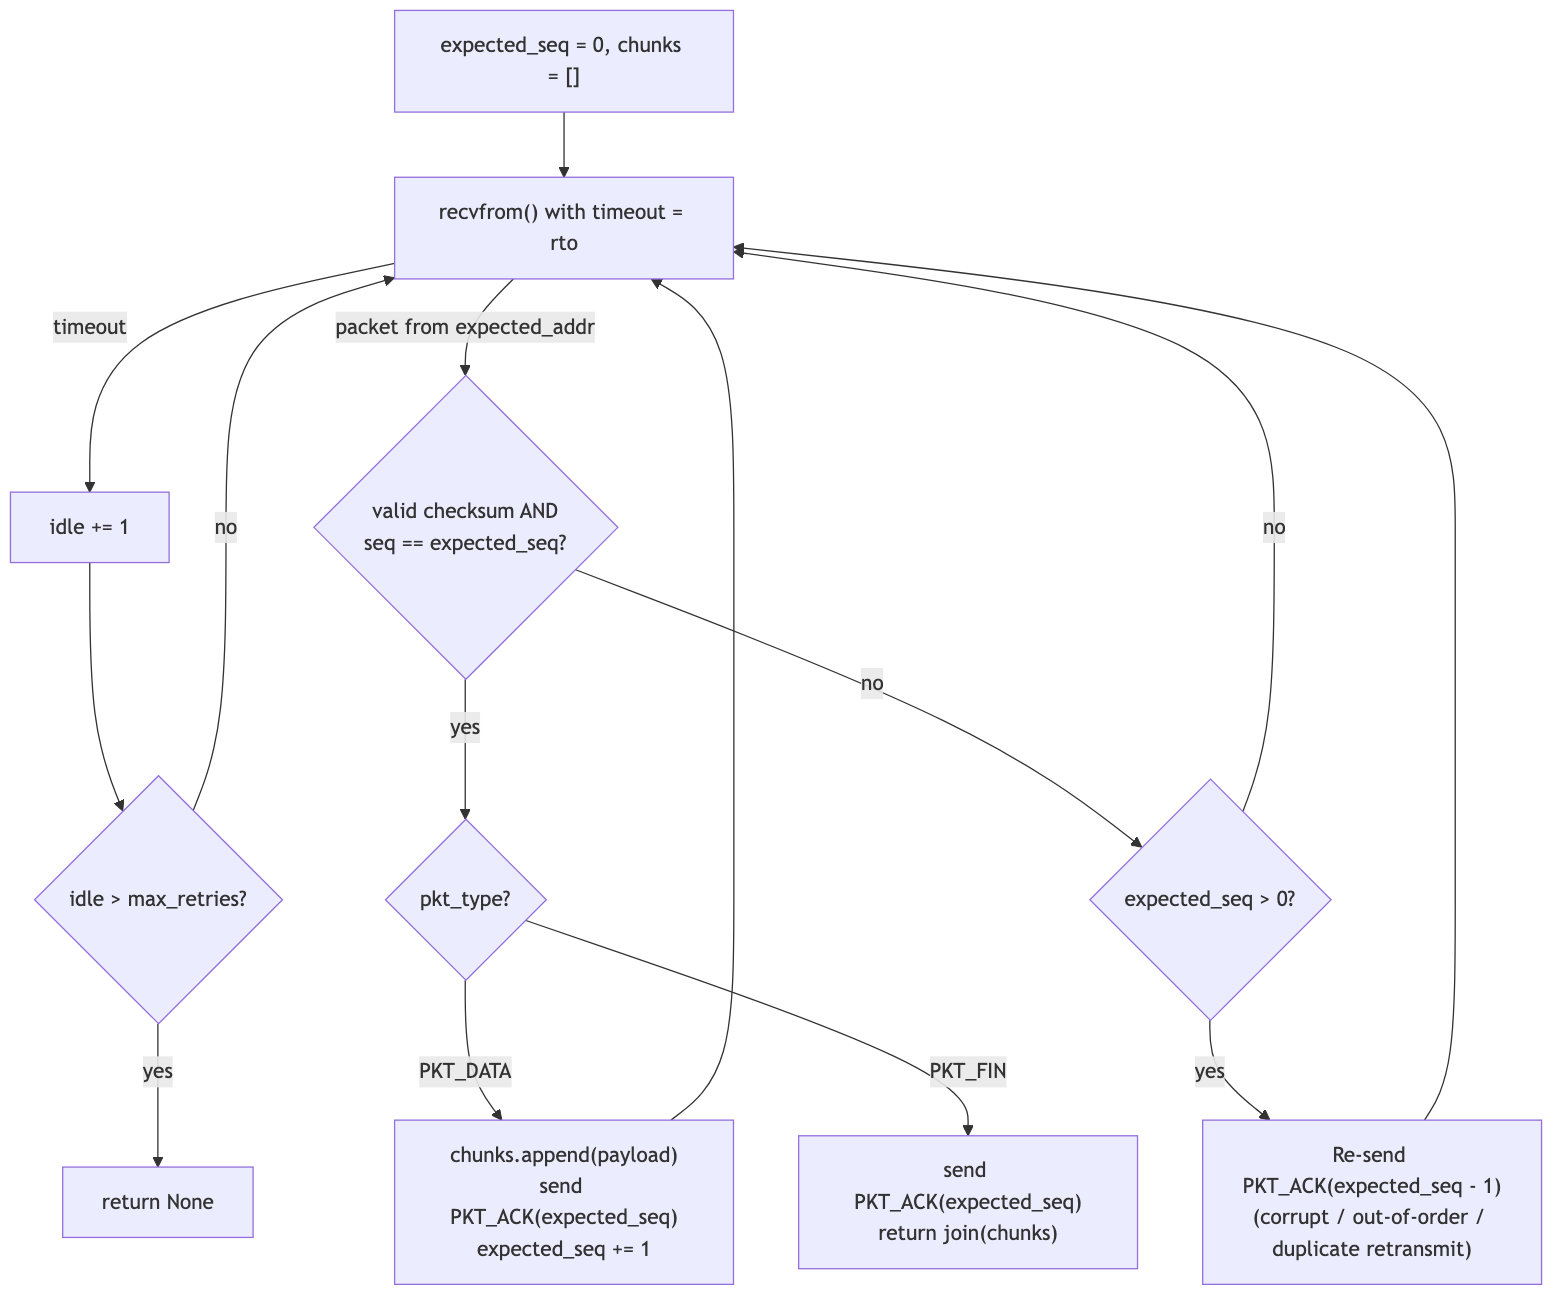
\includegraphics[width=0.78\textwidth,height=0.8\textheight,keepaspectratio]{05_flowchart_gbn_receiver.png}
    \caption{Go-Back-N receiver state machine. Only strictly in-order packets are
             accepted and buffered; anything else re-triggers the last known-good
             cumulative ACK.}
    \label{fig:flow-gbn-receiver}
\end{figure}

\clearpage
\subsection{Client Data-Mode Selection}

Figure~\ref{fig:flow-mode-select} shows how the client picks its data-channel mode
at login (from \texttt{config.ini}'s \texttt{[client] data\_mode} default), and how
it can still be switched live via the REPL's \texttt{active}/\texttt{passive}/\texttt{fixed}
commands mid-session -- a genuine runtime choice, not just a static configuration.

\begin{figure}[htbp]
    \centering
    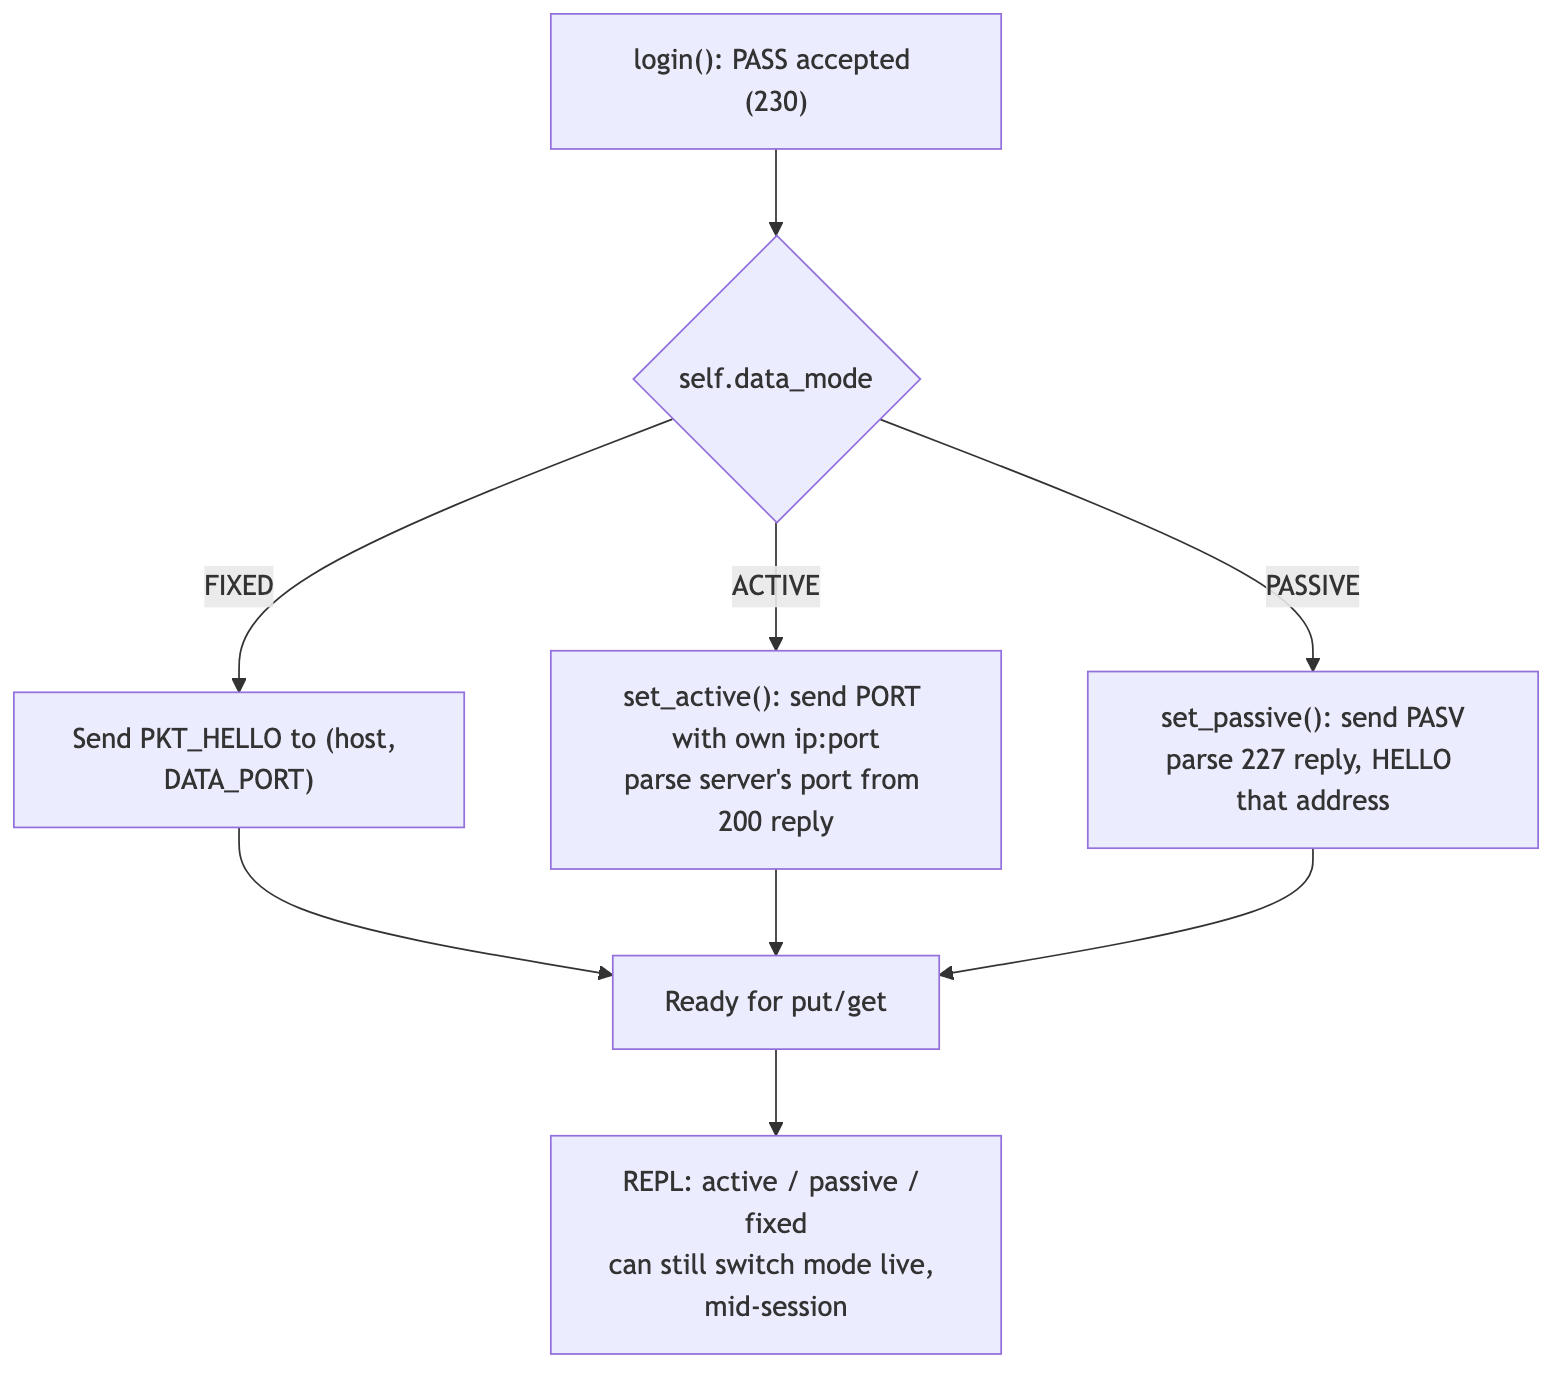
\includegraphics[width=0.7\textwidth,height=0.8\textheight,keepaspectratio]{06_flowchart_client_mode_select.png}
    \caption{Client data-mode selection and live switching.}
    \label{fig:flow-mode-select}
\end{figure}

\clearpage
\subsection{Design Rationale: RFC 959 Deviations}

\begin{itemize}
    \item \textbf{Active mode's server-port disclosure.} Real RFC~959 active mode
          does not need the server to report its own port back to the client,
          because TCP's server-initiated \texttt{connect()} reuses one bidirectional
          socket for both directions. This project's UDP data channel is
          connectionless, so the upload direction (\texttt{STOR} while in ACTIVE
          mode) needs an explicit destination port that the client cannot otherwise
          learn -- hence \texttt{Reply.port\_ok()} appends
          \texttt{"; server data port N"} to the \texttt{200} reply.
    \item \textbf{No control-channel negotiation for the reliability mode.} Unlike
          \texttt{data\_mode} (negotiated live via \texttt{PORT}/\texttt{PASV}),
          \texttt{[reliability] mode} (\texttt{none}/\texttt{gbn}) has no protocol
          command -- both ends must be configured identically ahead of time, the
          same way two TCP stacks must speak the same protocol version. This
          mirrors how TCP's reliability is transparent to the application layer,
          and avoids inventing a command outside the spec's approved command table
          (Section~2.2).
\end{itemize}

\clearpage
% ============================================================
\section{Task Assignment Matrix}
% ============================================================

% TODO(team): fill in real ownership before submission.
% Đã điều chỉnh lại một chút chiều rộng các cột để cân đối hơn
\begin{longtable}{@{}p{5cm}p{4cm}p{4.5cm}@{}}
\toprule
\textbf{Module / Component} & \textbf{Owner} & \textbf{Collaborators / Reviewers} \\
\midrule
\endhead % Khai báo phần đầu bảng sẽ được lặp lại nếu sang trang mới

Control channel (\texttt{server.py} command dispatch, \texttt{common.py} line protocol) & \_\_\_\_\_\_\_\_ & \_\_\_\_\_\_\_\_ \\
Basic Level data channel (FIXED mode, \texttt{STOR}/\allowbreak\texttt{RETR}) & \_\_\_\_\_\_\_\_ & \_\_\_\_\_\_\_\_ \\
% Thêm \allowbreak để cho phép xuống dòng ở các dấu /
Directory tree (\texttt{CWD}/\allowbreak\texttt{MKD}/\allowbreak\texttt{RMD}/\allowbreak\texttt{LIST}/\allowbreak\texttt{NLST}/\allowbreak\texttt{STAT}/\allowbreak\texttt{MDTM}) & \_\_\_\_\_\_\_\_ & \_\_\_\_\_\_\_\_ \\
Active/Passive mode (\texttt{PORT}/\allowbreak\texttt{PASV}), incl. the Passive port-range fix (\texttt{passive\_port\_min}/\allowbreak\texttt{passive\_port\_max}) & Le Kim Chau & Doan Cong Pho \\
Concurrency (multi-threading, active session table) & \_\_\_\_\_\_\_\_ & \_\_\_\_\_\_\_\_ \\
Go-Back-N reliable-UDP layer (\texttt{common.gbn\_send}/\allowbreak\texttt{gbn\_receive}) & Doan Cong Pho & Le Kim Chau \\
External deployment (Azure VM setup, NSG inbound rules) & Doan Cong Pho & Le Kim Chau \\
Integrity verification (\texttt{HASH}, \texttt{compute\_hash}) & \_\_\_\_\_\_\_\_ & \_\_\_\_\_\_\_\_ \\
Configuration layer (\texttt{config.py}/\allowbreak\texttt{config.ini}) & \_\_\_\_\_\_\_\_ & \_\_\_\_\_\_\_\_ \\
Client REPL (\texttt{client.py}) & \_\_\_\_\_\_\_\_ & \_\_\_\_\_\_\_\_ \\
Testing \& demo evidence & \_\_\_\_\_\_\_\_ & \_\_\_\_\_\_\_\_ \\
Technical report \& diagrams & \_\_\_\_\_\_\_\_ & \_\_\_\_\_\_\_\_ \\
\bottomrule
\end{longtable}
\textit{Note: per Section 4.1 of the project spec, individual grades are
determined by this matrix, peer evaluation, and targeted oral-viva questions --
each member should be able to explain their assigned module's code in detail,
independent of whether AI assistance was used to help write it (Section 4.2).}

\clearpage
% ============================================================
\section{Self-Assessment \& Peer Evaluation}
% ============================================================

\subsection*{Doan Cong Pho -- Self-Assessment}
Focused on the Excellent Level reliable-UDP layer and external deployment.
Learned to reason concretely about the UDP-vs-RUDP trade-off rather than treating
``reliable'' as a free upgrade: plain UDP (\texttt{[reliability] mode = none}) never
guarantees a file arrives intact -- a single lost datagram silently corrupts the
transfer, as demonstrated in Section~7.1 -- while Go-Back-N trades that risk for
throughput: every retransmission is a full window resend, and the sliding-window
size directly controls how much that trade-off costs under loss. Also set up and
maintained the external Azure VM (\texttt{pho-vir}) used for real-network testing
(Section~7.2) and configured its inbound NSG rules, including opening a dedicated
port range for Passive/Active mode traffic.

% TODO(Pho): add specifics -- challenges encountered while implementing/testing
% Go-Back-N, and an honest assessment of which AI-assisted parts you can defend
% unaided in the oral viva (per spec Section 4.2's zero-tolerance policy).

\subsection*{Le Kim Chau -- Self-Assessment}
Focused on Advanced Level Active/Passive mode and its real-world failure modes.
Learned that Active mode (\texttt{PORT}) breaks down when the client sits behind a
firewall or NAT, since the server has to initiate an inbound connection to a port
the client's own NAT never opened a mapping for -- a problem no amount of
client-side configuration fixes. Diagnosed and fixed the corresponding Passive-mode
gap: binding each session's UDP socket to a random OS-assigned port worked on
loopback but broke on the VM, because a cloud NSG/firewall can't sensibly allow
``any random port''; the fix was constraining Passive/Active sockets to a fixed,
configurable range (\texttt{passive\_port\_min}/\texttt{passive\_port\_max} in
\texttt{config.ini}) so only that range needs to be opened once (Section~7.2).

% TODO(Chau): add specifics -- challenges encountered, and an honest assessment of
% which AI-assisted parts you can defend unaided in the oral viva.

\subsection*{Peer Evaluation}
% TODO(team): each member writes a short evaluation of the other's contribution
% (spec Section 4.1 -- individual grades depend on this, not just the group's
% working code).
\textit{[To be completed by each member.]}

\begin{table}[htbp]
\centering
\caption{Agreed contribution percentages}
\begin{tabular}{@{}ll@{}}
\toprule
\textbf{Member} & \textbf{Contribution \%} \\
\midrule
Doan Cong Pho & 50\% \\
Le Kim Chau   & 50\% \\
\midrule
\textbf{Total} & \textbf{100\%} \\
\bottomrule
\end{tabular}
\end{table}

\clearpage
% ============================================================
\section{GenAI Usage \& Code Refinement Log}
% ============================================================

Please check out this GitHub link for the GenAI usage prompts and code refinement log:
\url{https://github.com/your-username/your-repo-link}



\clearpage
% ============================================================
\section{Application Demo Evidence}
% ============================================================

\subsection{Reliable-UDP vs. Best-Effort UDP: File Integrity Under Loss}

To make the practical difference between \texttt{[reliability] mode = none} and
\texttt{mode = gbn} concrete, the same 2816$\times$1536 JPEG-in-PNG image
(\texttt{heavy\_pic.png}, 9{,}475{,}477 bytes) was uploaded and downloaded once
over each mode under identical real-world network conditions where UDP datagram
loss occurred.

\begin{table}[htbp]
\centering
\caption{Byte-level comparison of the two transferred files}
\begin{tabular}{@{}lrr@{}}
\toprule
& \textbf{Go-Back-N (\texttt{mode=gbn})} & \textbf{Best-effort (\texttt{mode=none})} \\
\midrule
File size & 9{,}475{,}477 bytes & 8{,}272{,}277 bytes \\
Matches source & Yes (byte-identical) & No \\
First divergence & --- & Offset 3{,}399{,}680 (= chunk \#3320 $\times$ 1024B) \\
Missing data & 0 bytes & 1{,}203{,}200 bytes (= 1175 $\times$ 1024B chunks) \\
\bottomrule
\end{tabular}
\end{table}

Both files are byte-identical up to offset 3{,}399{,}680 -- exactly a multiple of
\texttt{CHUNK\_SIZE} (1024 bytes) -- confirming the divergence corresponds to whole
UDP datagrams, not partial corruption within a packet (each packet's CRC32
checksum, verified in \texttt{common.parse\_packet()}, rules that out). Under
\texttt{mode = none}, \texttt{handle\_stor()}'s receive loop stores each chunk in a
dict keyed by sequence number and reassembles via
\texttt{"".join(chunks[seq] for seq in sorted(chunks))} -- any sequence numbers that
never arrived are silently \emph{skipped} rather than padded, so the file is not
merely truncated at the end but shifted/corrupted from the point of the first loss
onward, exactly as visible in Figure~\ref{fig:evidence-udp}.

\begin{figure}[htbp]
    \centering
    
\includegraphics[width=0.85\textwidth,height=0.8\textheight,keepaspectratio]{evidence_rudp.jpg}
    \caption{Downloaded via \texttt{mode = gbn} -- fully intact, matches the source
             file byte-for-byte (confirmed via \texttt{diff} and SHA-256 comparison
             through the \texttt{HASH} command).}
    \label{fig:evidence-rudp}
\end{figure}

\begin{figure}[htbp]
    \centering
    
\includegraphics[width=0.85\textwidth,height=0.8\textheight,keepaspectratio]{evidence_udp.jpg}
    \caption{Downloaded via \texttt{mode = none} (best-effort) -- the top portion
             decodes correctly, then the image cuts to blank exactly where the lost
             chunk's data should have continued. This is the documented,
             deliberate Basic/Advanced Level limitation that Go-Back-N (Excellent
             Level) exists to solve.}
    \label{fig:evidence-udp}
\end{figure}

\clearpage
\subsection{External Deployment Evidence (Azure VM)}

All of the above is reproducible on loopback, but loopback cannot exercise the
scenarios that actually motivate this project's design decisions -- NAT traversal
for \texttt{PASV}'s \texttt{advertise\_ip}, firewall/NSG port restrictions for the
Active/Passive per-session sockets, and real (non-zero) latency/loss on the wire.
The group additionally deployed and tested the server on an external Azure VM
(\texttt{pho-vir}), the same VM used for the original Basic Level cross-machine
demo documented in \texttt{docs/GENAI\_LOG.md} (Entries 3--9), reachable from a
separate client machine over the public internet rather than \texttt{127.0.0.1}.

\begin{figure}[htbp]
    \centering
    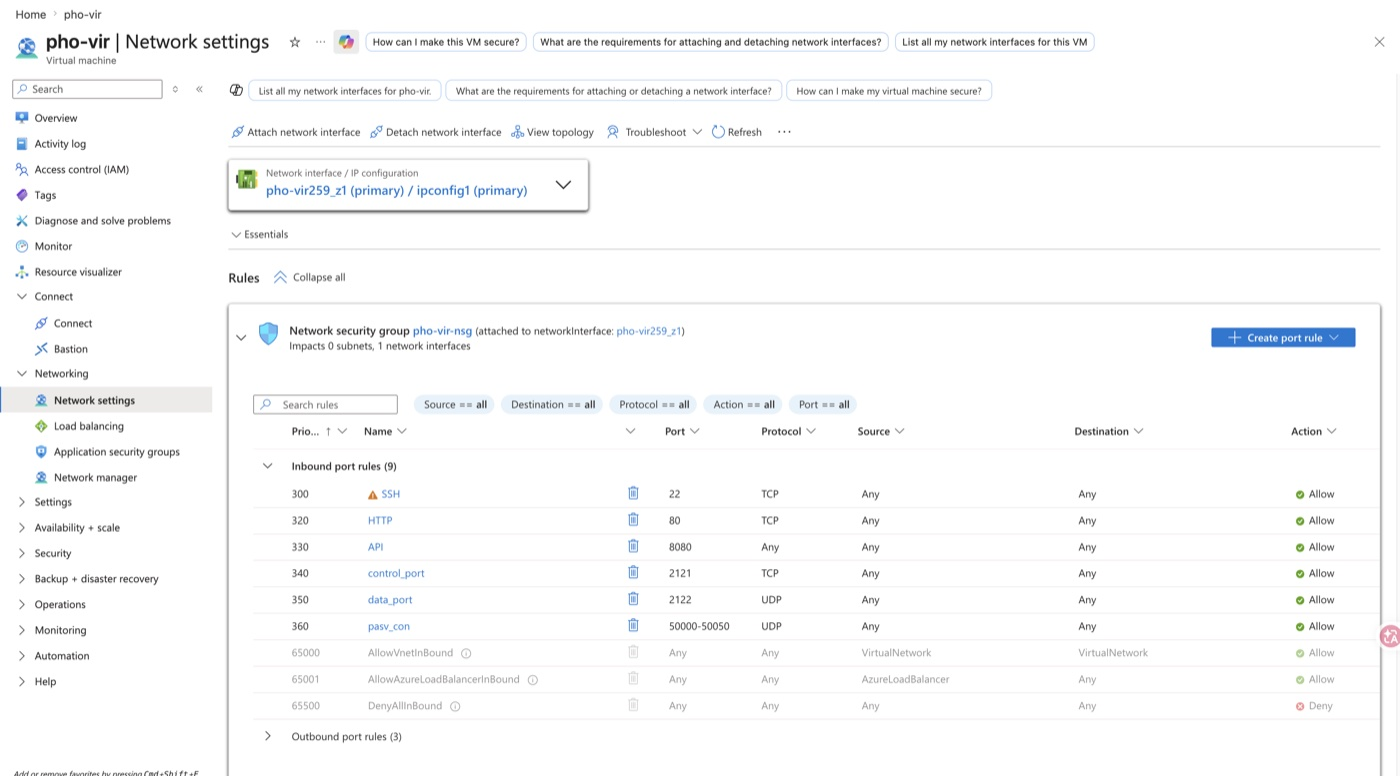
\includegraphics[width=0.95\textwidth]{evidence_azure_nsg.jpg}
    \caption{Azure Network Security Group (\texttt{pho-vir-nsg}) inbound rules for
             the deployment VM. \texttt{control\_port} (2121/TCP) and
             \texttt{data\_port} (2122/UDP) are the Basic Level control/FIXED-mode
             ports; \texttt{pasv\_con} (50000--50050/UDP) is the Advanced/Excellent
             Level Active/Passive per-session port range, matching
             \texttt{config.ini}'s \texttt{passive\_port\_min}/\texttt{passive\_port\_max}
             exactly (Section 3 of this report, and the README's ``Configuration''
             section) -- opened specifically so PASV/PORT-mode sessions are
             reachable from outside the VM without exposing an arbitrary
             OS-assigned ephemeral port per session.}
    \label{fig:evidence-azure-nsg}
\end{figure}

This is what closes the loop on the \texttt{advertise\_ip}/NAT problem discussed
earlier in the project (a PASV server behind NAT that announces its private IP is
unreachable from an external client) -- \texttt{config.ini}'s
\texttt{advertise\_ip} is set to the VM's public IP, and Figure~\ref{fig:evidence-azure-nsg}
confirms the corresponding inbound path is actually open, not just configured.

\subsubsection{Live capture: real packet loss over the VM path, Basic Level (\texttt{mode = none})}

The following is an unedited client/server transcript from an actual interactive
session against \texttt{pho-vir} (client on a home network, server on the Azure VM,
\texttt{[reliability] mode = none} -- i.e. plain Basic Level FIXED mode, no Advanced
or Excellent Level techniques involved). Both sides report success, but the byte
counts do not match:

\begin{lstlisting}
--- client ---
ftp> put client_files/baby_crying.jpg
150 File status okay, opening data connection.
226 Transfer complete.
ftp> get baby_crying.jpg
150 File status okay, opening data connection.
[+] Saved to .../client_downloads/baby_crying.jpg (69833 bytes)
226 Transfer complete.

--- server (pho-vir) ---
[('116.111.185.192', 10947)] STOR baby_crying.jpg
[+] Stored 'baby_crying.jpg' (89289 bytes) from user 'alice'
[('116.111.185.192', 10947)] RETR baby_crying.jpg
[+] Sent 'baby_crying.jpg' (89289 bytes) to user 'alice'
\end{lstlisting}

The server sent 89{,}289 bytes; the client saved 69{,}833 -- a shortfall of
19{,}456 bytes (exactly 19 $\times$ \texttt{CHUNK\_SIZE}, 1024 bytes each: 19 whole
UDP datagrams lost over the real internet path, roughly 21.8\% of the transfer),
yet \emph{both} sides printed \texttt{226 Transfer complete.} Independently
re-verified on disk after the session:
\begin{lstlisting}
$ ls -la client_files/baby_crying.jpg client_downloads/baby_crying.jpg
-rw-r--r--  89289  client_files/baby_crying.jpg
-rw-r--r--  69833  client_downloads/baby_crying.jpg
$ diff client_files/baby_crying.jpg client_downloads/baby_crying.jpg
Binary files ... differ
$ file client_downloads/baby_crying.jpg
client_downloads/baby_crying.jpg: JPEG image data, ... baseline, precision 8, 590x738, components 3
\end{lstlisting}
\texttt{file} still identifies it as a JPEG (a truncated JPEG's header is still
well-formed even when the scan data mid-stream is missing), which is precisely
why byte-count/checksum verification -- not "does it look like an image file" --
is the correct integrity check, and precisely the gap \texttt{HASH}
(Section~7.1) and Go-Back-N exist to close: under \texttt{mode = none}, neither
\texttt{handle\_stor()}/\texttt{handle\_retr()} on the server nor
\texttt{\_recv\_data\_payload()} on the client verify that every sequence number
0..N-1 was actually received before declaring success -- the receive loop simply
stops as soon as a \texttt{PKT\_FIN} arrives, regardless of how many
\texttt{PKT\_DATA} packets never did. Re-running the identical \texttt{put}/\texttt{get}
with \texttt{[reliability] mode = gbn} on both ends (Section~7.1's controlled test)
is the documented fix -- \texttt{gbn\_send()} does not return success until the
receiver has cumulatively ACKed every packet including the final \texttt{FIN}.

\clearpage
\subsection{Verified Test Sessions (Terminal Transcripts)}

Rather than static screenshots, the transcripts below are captured directly from
real client/server sessions run against the actual codebase during development
verification (loopback, \texttt{127.0.0.1}) -- copy-pasteable, and reproducible by
re-running the same commands per README.md's ``Running'' section. Each corresponds
to one item from spec Section 4.5's demo checklist.

\subsubsection{Basic Level: ASCII put/get round-trip}
\begin{lstlisting}
$ printf 'user alice\npass password123\nput /tmp/basic_test.txt\nget basic_test.txt\nquit\n' | python3 client.py 127.0.0.1
220 Service ready.
ftp> 331 Username OK, need password.
ftp> 230 Login successful.
ftp> 150 File status okay, opening data connection.
226 Transfer complete.
ftp> 150 File status okay, opening data connection.
[+] Saved to client_downloads/basic_test.txt (33 bytes)
226 Transfer complete.
ftp> 221 Goodbye.

$ diff /tmp/basic_test.txt client_downloads/basic_test.txt && echo "DIFF-OK: files identical"
DIFF-OK: files identical
\end{lstlisting}

\subsubsection{Advanced Level: directory tree operations}
\begin{lstlisting}
ftp> mkd sub
257 "/sub" created.
ftp> cwd sub
250 Directory changed to "/sub".
ftp> pwd
257 "/sub"
ftp> put /tmp/basic_test.txt
150 File status okay, opening data connection.
226 Transfer complete.
ftp> ls
150 File status okay, opening data connection.
-rw-r--r--         33 basic_test.txt
226 Transfer complete.
ftp> cdup
250 Directory changed to "/".
ftp> ls
150 File status okay, opening data connection.
-rw-r--r--         33 basic_test.txt
drwxr-xr-x          0 sub
226 Transfer complete.
ftp> stat sub/basic_test.txt
213 file 33 bytes
ftp> mdtm sub/basic_test.txt
213 20260724015402
\end{lstlisting}

\subsubsection{Advanced Level: binary transfer, Passive and Active mode}
\begin{lstlisting}
ftp> type I
200 Command OK.
ftp> passive
227 Entering Passive Mode (127,0,0,1,207,104).
[*] Data mode: PASSIVE (server at 127.0.0.1:53096)
ftp> put /tmp/binary_test.bin
150 File status okay, opening data connection.
226 Transfer complete.
ftp> get binary_test.bin /tmp/binary_out_pasv.bin
150 File status okay, opening data connection.
[+] Saved to /tmp/binary_out_pasv.bin (5000 bytes)
226 Transfer complete.

$ diff /tmp/binary_test.bin /tmp/binary_out_pasv.bin && echo "PASSIVE binary DIFF-OK"
PASSIVE binary DIFF-OK

--- Active mode, second user ---
ftp> active
200 PORT command successful; server data port 63898.
[*] Data mode: ACTIVE (server will use port 63898)
ftp> put /tmp/binary_test.bin bin_active.bin
150 File status okay, opening data connection.
226 Transfer complete.
ftp> get bin_active.bin /tmp/binary_out_active.bin
150 File status okay, opening data connection.
[+] Saved to /tmp/binary_out_active.bin (5000 bytes)
226 Transfer complete.

$ diff /tmp/binary_test.bin /tmp/binary_out_active.bin && echo "ACTIVE binary DIFF-OK"
ACTIVE binary DIFF-OK
\end{lstlisting}

\subsubsection{Advanced Level: concurrency -- two simultaneous clients, active session table}
Two client processes (\texttt{alice}, \texttt{bob}) run \texttt{put}+\texttt{get}
\emph{simultaneously} in Passive mode against the real Azure VM server
(\texttt{pho-vir}, \texttt{threading = thread}), each getting an independent
per-session UDP port from the configured \texttt{passive\_port\_min}--\texttt{passive\_port\_max}
range:
\begin{lstlisting}
--- alice ---
220 Service ready.
ftp> user alice
331 Username OK, need password.
ftp> pass password123
230 Login successful.
ftp> passive
227 Entering Passive Mode (20,249,210,239,195,80).
[*] Data mode: PASSIVE (server at 20.249.210.239:50000)
ftp> put alice_file.txt
150 File status okay, opening data connection.
226 Transfer complete.
ftp> get alice_file.txt
150 File status okay, opening data connection.
[+] Saved to .../alice_out.txt (68 bytes)
226 Transfer complete.
ftp> quit
221 Goodbye.

--- bob (run at the same time as alice, not sequentially) ---
220 Service ready.
ftp> user bob
331 Username OK, need password.
ftp> pass hunter2
230 Login successful.
ftp> passive
227 Entering Passive Mode (20,249,210,239,195,81).
[*] Data mode: PASSIVE (server at 20.249.210.239:50001)
ftp> put bob_file.txt
150 File status okay, opening data connection.
226 Transfer complete.
ftp> get bob_file.txt
150 File status okay, opening data connection.
[+] Saved to .../bob_out.txt (66 bytes)
226 Transfer complete.
ftp> quit
221 Goodbye.

$ diff alice_file.txt alice_out.txt && echo "ALICE OK"
ALICE OK
$ diff bob_file.txt bob_out.txt && echo "BOB OK"
BOB OK
\end{lstlisting}
Note the two independent ports allocated from the PASV range -- \texttt{50000}
for alice, \texttt{50001} for bob -- confirming each session got its own
dedicated per-session UDP socket rather than sharing one, which is what makes
running both \texttt{put}/\texttt{get} pairs genuinely concurrently (not just
back-to-back) safe.
The corresponding server-side console log, captured live on the VM during this
same run:
\begin{lstlisting}
azureuser@pho-vir:~/ip/hybrid_ftp$ python3 server.py
[*] Hybrid FTP server listening on TCP 2121, UDP data port 2122
[*] Concurrency mode: thread
[+] Connection #1 from ('42.115.42.57', 7957)
[+] Connection #2 from ('42.115.42.57', 59695)
[*] Active sessions:
      #1  42.115.42.57:7957   user=None  mode=FIXED  cwd=/
      #2  42.115.42.57:59695  user=None  mode=FIXED  cwd=/
[('42.115.42.57', 7957)] USER bob
[('42.115.42.57', 59695)] USER alice
[('42.115.42.57', 7957)] PASS hunter2
[('42.115.42.57', 59695)] PASS password123
[*] Active sessions:
      #1  42.115.42.57:7957   user='bob'    mode=FIXED  cwd=/
      #2  42.115.42.57:59695  user='alice'  mode=FIXED  cwd=/
[('42.115.42.57', 59695)] PASV
[('42.115.42.57', 7957)] PASV
[*] Active sessions:
      #1  42.115.42.57:7957   user='bob'    mode=PASSIVE  cwd=/
      #2  42.115.42.57:59695  user='alice'  mode=PASSIVE  cwd=/
[('42.115.42.57', 59695)] STOR alice_file.txt
[('42.115.42.57', 7957)] STOR bob_file.txt
[+] Stored 'alice_file.txt' (68 bytes) from user 'alice'
[+] Stored 'bob_file.txt' (66 bytes) from user 'bob'
[('42.115.42.57', 7957)] RETR bob_file.txt
[+] Sent 'bob_file.txt' (66 bytes) to user 'bob'
[('42.115.42.57', 59695)] RETR alice_file.txt
[+] Sent 'alice_file.txt' (68 bytes) to user 'alice'
[('42.115.42.57', 7957)] QUIT
[*] Active sessions:
      #2  42.115.42.57:59695  user='alice'  mode=PASSIVE  cwd=/
[*] Session #1 for ('42.115.42.57', 7957) (user='bob') closed.
[('42.115.42.57', 59695)] QUIT
[*] Active sessions:
      (none)
[*] Session #2 for ('42.115.42.57', 59695) (user='alice') closed.
\end{lstlisting}
Two details in this log, beyond the active-session table itself, are direct
evidence of genuine concurrency rather than fast sequential handling: (1)
\texttt{STOR alice\_file.txt} (session \#2) and \texttt{STOR bob\_file.txt}
(session \#1) are both logged \emph{before either ``Stored'' confirmation
appears} -- under \texttt{threading = single} this would be impossible, since
one session's \texttt{handle\_stor()} call would have to fully return before
the next connection could even be accepted; and (2) each session independently
negotiates \texttt{PASV} and transitions \texttt{FIXED} $\to$ \texttt{PASSIVE}
without affecting the other's row in the table, confirming the per-session
state (\texttt{Session.data\_mode}, \texttt{Session.data\_sock}) is correctly
isolated per connection, not shared global state.

Both transfers completed with independent, uncorrupted data -- confirming
per-session UDP socket isolation under concurrency (Section 3 of this report;
FIXED mode does not provide this isolation, by design -- see the README's
``Concurrency'' section).

\subsubsection{Excellent Level: Go-Back-N transfer with automatic hash verification (live, Azure VM)}
Run against the real \texttt{pho-vir} VM (both ends set to
\texttt{[reliability] mode = gbn}, \texttt{[integrity] verify = true}) -- a
20{,}000-byte random binary file, \texttt{put} then \texttt{get}, with automatic
hash verification after each:
\begin{lstlisting}
--- client ---
220 Service ready.
ftp> user alice
331 Username OK, need password.
ftp> pass password123
230 Login successful.
ftp> put gbn_test.bin
150 File status okay, opening data connection.
226 Transfer complete.
[+] Integrity verified (sha256): MATCH (5d579fe17ea2fa6ccb0a964604b50d68a0029e2628979e8d49b70d64c380db84)
ftp> get gbn_test.bin
150 File status okay, opening data connection.
[+] Saved to .../gbn_test_out.bin (20000 bytes)
226 Transfer complete.
[+] Integrity verified (sha256): MATCH (5d579fe17ea2fa6ccb0a964604b50d68a0029e2628979e8d49b70d64c380db84)
ftp> hash gbn_test.bin
213 sha256 5d579fe17ea2fa6ccb0a964604b50d68a0029e2628979e8d49b70d64c380db84
ftp> quit
221 Goodbye.

$ diff gbn_test.bin gbn_test_out.bin && echo "GBN-VM DIFF-OK"
GBN-VM DIFF-OK

--- server (pho-vir) ---
[*] Hybrid FTP server listening on TCP 2121, UDP data port 2122
[*] Concurrency mode: thread
[+] Connection #1 from ('42.115.42.57', 1823)
[('42.115.42.57', 1823)] USER alice
[('42.115.42.57', 1823)] PASS password123
[('42.115.42.57', 1823)] STOR gbn_test.bin
[+] Stored 'gbn_test.bin' (20000 bytes) from user 'alice'
[('42.115.42.57', 1823)] HASH gbn_test.bin
[('42.115.42.57', 1823)] RETR gbn_test.bin
[+] Sent 'gbn_test.bin' (20000 bytes) to user 'alice'
[('42.115.42.57', 1823)] HASH gbn_test.bin
[('42.115.42.57', 1823)] HASH gbn_test.bin
[('42.115.42.57', 1823)] QUIT
[*] Session #1 for ('42.115.42.57', 1823) (user='alice') closed.
\end{lstlisting}
This is the same \texttt{put}/\texttt{get} pair as the Basic Level live-capture
in Section~7.2, over the same real network path where 21.8\% packet loss was
observed under \texttt{mode = none} -- here, with \texttt{mode = gbn}, the
transfer is byte-identical (\texttt{diff}-confirmed) and hash-verified twice
independently (once automatically after each transfer, once via a manual
\texttt{hash} query), with no manual retry needed. The three \texttt{HASH}
entries in the server log correspond to: the automatic post-\texttt{put} check,
the automatic post-\texttt{get} check, and the explicit \texttt{hash gbn\_test.bin}
command -- all against the one file stored server-side, confirming
\texttt{HASH} is idempotent and side-effect-free (querying it repeatedly
doesn't alter or re-transfer the file).

\texttt{HASH} was also separately confirmed to be content-sensitive rather than
trivially always matching, by querying it against a different file on the
server and observing a different digest (\texttt{94b306c8...} vs.
\texttt{5d579fe1...}), proving the client's \texttt{MATCH}/\texttt{MISMATCH}
comparison is a real byte-level check, not a stub.

\subsubsection{Excellent Level: Go-Back-N recovery under controlled, simulated packet loss}
Whether the live VM run above needed a retransmission at all isn't known from
that transcript alone (no retransmit logging existed at the time it was
captured -- added afterward, see Section~7.3.7) -- to directly prove the
retransmit path itself is correct, not just that the happy path works, this
test adversarially forces loss under controlled conditions rather than waiting
for the real internet to cooperate. Isolated \texttt{gbn\_send()}/\texttt{gbn\_receive()}
trials against a UDP socket
wrapper that randomly drops both DATA and ACK packets (10--50\% simultaneous
bidirectional loss; full harness described in the GenAI log, Entry 12):
\begin{lstlisting}
  payload=  8000B drop=15% ... -> PASS   (x10 repeated trials, different seeds)
  10/10 no-false-positive (expect 10/10)

  payload=  1024B drop=50% window=4 -> sender_ok=True bytes_match=True -> PASS

ALL TRIALS PASSED (no false positives, ever)
\end{lstlisting}
The property verified is the one that matters for an RDT layer: \texttt{gbn\_send()}
never reports success unless the data was actually reassembled correctly --
confirmed across every trial, not just the happy path.

\subsubsection{Live retransmission logging over the Azure VM path}
\texttt{gbn\_send()} and \texttt{gbn\_receive()} were extended with optional
logging callbacks, wired in \texttt{server.py} and \texttt{client.py} to print
a console line whenever a real retransmission actually fires -- making loss
recovery directly observable instead of only inferable from end-to-end
success. A 3{,}000{,}000-byte random file (\texttt{window\_size = 4}, so
$\sim$2930 packets) was transferred \texttt{put} then \texttt{get} against
the VM; the download surfaced two genuine retransmissions:
\begin{lstlisting}
--- client ---
ftp> get huge_file.bin
150 File status okay, opening data connection.
[GBN] out-of-order/duplicate/corrupt from ('20.249.210.239', 2122) (expected seq=1580, got=1576) -- re-ACKing 1579
[GBN] out-of-order/duplicate/corrupt from ('20.249.210.239', 2122) (expected seq=1580, got=1577) -- re-ACKing 1579
[GBN] out-of-order/duplicate/corrupt from ('20.249.210.239', 2122) (expected seq=1580, got=1578) -- re-ACKing 1579
[GBN] out-of-order/duplicate/corrupt from ('20.249.210.239', 2122) (expected seq=1580, got=1579) -- re-ACKing 1579
[+] Saved to .../huge_file_out.bin (3000000 bytes)
226 Transfer complete.
[+] Integrity verified (sha256): MATCH (ab50e9dd32429ada403af542f0d1acf829c4d3a2aec19488ec461cd92f6737a8)

--- server (pho-vir) ---
[('42.115.42.57', 63034)] RETR huge_file.bin
[GBN] retransmit window seq=1576..1579 (retry #1) to ('42.115.42.57', 23994) -- real packet loss detected
[GBN] retransmit window seq=2424..2427 (retry #1) to ('42.115.42.57', 23994) -- real packet loss detected
[+] Sent 'huge_file.bin' (3000000 bytes) to user 'alice'

$ diff huge_file.bin huge_file_out.bin && echo "HUGE-FILE DIFF-OK"
HUGE-FILE DIFF-OK
\end{lstlisting}
The two retransmissions demonstrate \emph{different} failure modes, both
handled correctly:
\begin{itemize}
    \item \textbf{seq 1576--1579}: the client's log shows these exact packets
          being logged as \emph{duplicates} -- already received, with
          \texttt{expected\_seq} already advanced past them. This means the
          original DATA delivery succeeded,
          but the client's \emph{ACK} for it was lost on the return path,
          so the server's RTO fired needlessly. The client's re-ACK of 1579
          (cumulative) eventually got through, letting the server's window
          slide -- redundant network traffic, zero data corruption.
    \item \textbf{seq 2424--2427}: no corresponding duplicate line appears in
          the client log for this range, meaning these packets were
          genuinely new on arrival -- the original DATA itself was lost, and
          the retransmission delivered it for the first time.
\end{itemize}
Both cases resolved without any manual intervention, and the final file is
still byte-identical and hash-verified -- this is the direct, observed-in-
the-wild counterpart to the controlled loss simulation in Section~7.3.6, over
the same real network path where 21.8\% loss was measured under
\texttt{mode = none} in Section~7.2.

\end{document}